% !TEX TS-program = xelatex
\documentclass[12pt]{article}
\usepackage{amsthm,amsmath,amssymb,braket,graphicx,enumitem,booktabs,multirow,booktabs,wrapfig,cancel,caption,fancyhdr,relsize,textpos,booktabs,tocbibind,titlesec,color}
\usepackage[top=0.5in]{geometry}
\usepackage[T1]{fontenc}
\usepackage[pdfusetitle]{hyperref}
\renewcommand{\arraystretch}{2}
\setlength\delimitershortfall{-2pt}
\setcounter{tocdepth}{1}
\DeclareMathOperator{\sech}{sech}
\raggedbottom
\numberwithin{equation}{section}
\allowdisplaybreaks

\title{The Tight-Binding Model on the 2D Lattice\vspace*{-30pt}}
\author{}
\begin{document}
\maketitle
\subsection*{Single-particle Hamiltonian viewpoint}
This method deals with the situation in which the local atomic orbitals are a good approximation to the full problem, and fairly good solutions can be obtained by adding corrections to the local wavefunctions. We start by separating the full Hamiltonian into a local and a non-local piece:
\begin{equation}\begin{aligned}
	H = \sum_i H_i + H_\text{nloc}
\end{aligned}\end{equation}
$H_i$ is an operator that acts only very close to the real space lattice site \(i\), and is zero otherwise. A very extreme and simple example would be a chemical potential term:
\begin{equation}\begin{aligned}
	H_i = \mu \sum_{\sigma} \hat n_{i\sigma}
\end{aligned}\end{equation}
where \(\hat n_{i\sigma} = c^\dagger_{i \sigma}c_{i \sigma}\) is thee number operator for the $i^\text{th}$ site.
A more non-trivial example would be an extremely localised Coulomb repulsion term:
\begin{equation}\begin{aligned}
	H_i =  U\hat n_{i \uparrow}\hat n_{i \downarrow}
\end{aligned}\end{equation}
The non-local piece $H_\text{nloc}$ connects multiple sites. A simple example of such a term would be a nearest-neighbour hopping:
\begin{equation}\begin{aligned}
	H_\text{nloc} =  -t\sum_{i\sigma} \left(c^\dagger_{i\sigma}c_{i+1,\sigma} + \text{h.c.}\right)
\end{aligned}\end{equation}
In general, let $\left\{\ket{\Psi^n_i}\right\}$ be the set of eigenstates of the local Hamiltonian \(H_i\):
\begin{equation}\begin{aligned}
	H_i \ket{\Psi_i^n} = E^n_i\ket{\Psi_\text{loc}^n}
\end{aligned}\end{equation}
We will drop the superscript $i$ on the energy eigenvalue because they are actually independent of $i$ on account of translation invariance.
We assume that all the \(\psi_i^n(\vec r - \vec R_i)\) are very local; that is, they are non-zero only very close to their specific lattice sites \(\left( \vec r - \vec R_i \sim 0 \right) \). More specifically, we assume that \(\psi_i^n(\vec r)\) becomes zero when $H_\text{nloc}(\vec r - \vec R_i)$ is non-zero. In such a situation, \(\psi_i^n(\vec r - \vec R_i)\) becomes a very good wavefunction of the full Hamiltonian:
\begin{equation}\begin{aligned}
	H(\vec r)\psi_i^n(\vec r - \vec R_i) &= \left[\sum_i H_i(\vec r) + H_\text{nloc}(\vec r)\right] \psi_i^n(\vec r - \vec R_i)\\
					   &= \begin{cases}
						   H_i(\vec r)\psi_i^n(\vec r - \vec R_i) = E^n\psi_i^n(\vec r - \vec R_i) & \text{ when }\vec r \sim \vec R_i\\
						   H_\text{nloc}(\vec r) \psi_i^n(\vec r - \vec R_i) = 0 & \text{ when }\vec r \nsim \vec R_i\\
	\end{cases}
\end{aligned}\end{equation}
However, these wavefunctions do not satisfy Bloch's theorem. The following linear combination does:
\begin{equation}\begin{aligned}
	\phi^n(\vec k) = \frac{1}{\sqrt N}\sum_{i}e^{i \vec{k}\cdot\vec{R_i}}\psi^n_i(\vec r - \vec R_i)
\end{aligned}\end{equation}
because it can be rewritten as
\begin{equation}\begin{aligned}
	\phi^n(\vec k) = \frac{1}{\sqrt N}e^{i \vec{k}\cdot\vec{r}}\sum_{i}e^{-i \vec{k}\cdot\left(\vec r-\vec R_i\right)}\psi^n_i(\vec r - \vec R_i) = e^{i \vec{k}\cdot\vec{r}} u^n_{\vec k}(\vec r)
\end{aligned}\end{equation}
such that \(u^n_{\vec k}(\vec r)\) is translationally-invariant. The energy expectation values are
\begin{equation}\begin{aligned}
	\xi_{\vec k} = \bra{\Phi^n_{\vec k}}H\ket{\phi^n_{\vec k}} = \frac{1}{N}\sum_{ij}e^{i \vec k \cdot\left(\vec R_i - \vec R_j\right)}\bra{\Psi^n_i}H\ket{\Psi^n_j}
\end{aligned}\end{equation}
At this point we assume that the Hamiltonian has non-zero matrix elements for local and, at the most, nearest-neighbour terms:
\begin{equation}\begin{aligned}
	\bra{\Psi^n_i}H\ket{\Psi^n_j} = \alpha \delta_{ij} + \gamma \delta_{|i-j| - 1}
\end{aligned}\end{equation}
This gives
\begin{equation}\begin{aligned}
	\xi_{\vec k} = \alpha + \gamma\sum_{\vec e_i}e^{i \vec{ k}\cdot\vec{ e_i}}
\end{aligned}\end{equation}
\(\vec e_i\) runs over all vectors that connect a lattice site to its nearest neighbours. For a hypercubic lattice with spacings \(a_1, a_2, ...\), the expression becomes
\begin{equation}\begin{aligned}
	\xi_{\vec k} = \alpha + 2\gamma\sum_{i=x,y,...}\cos a_i k_i
\end{aligned}\end{equation}
\newpage
\subsection*{Second-quantized Hamiltonian viewpoint}
The tight-binding model can also be developed starting from a second-quantized Hamiltonian. Here we work with field operators:
\begin{equation}\begin{aligned}
	c_{\vec k}, c_{\vec q}^\dagger: \left\{ c_{\vec k}, c^\dagger_{\vec q} \right\} = \delta_{kq}
\end{aligned}\end{equation}
\(i,j\) are some quantum numbers. For example, \(c^\dagger(\vec r)\) creates an electron at position \(\vec r\).
\\\\
The assumption of at most nearest neighbour Hamiltonian matrix elements naturally leads to the model
\begin{equation}\begin{aligned}
	H = -t\sum_{\left<ij\right>, \sigma}\left(c^\dagger_{i \sigma}c_{j\sigma} + \text{h.c.}\right) - \mu \hat N
\end{aligned}\end{equation}
\(c^\dagger_{i\sigma}\) is the Fermionic field operator that creates an electron with spin \(\sigma\) at \(\vec R_i\). Defining the Foureir transforms as
\begin{equation}\begin{aligned}
	c^\dagger_{\vec k\sigma} = \frac{1}{\sqrt N}\sum_{i}e^{\vec{k}\cdot\vec{R_i}}c^\dagger_{i\sigma}, && c^\dagger_{i\sigma} = \frac{1}{\sqrt N}\sum_{i}e^{-\vec{k}\cdot\vec{R_i}}c^\dagger_{\vec k, \sigma}
\end{aligned}\end{equation}
Using this, we can write
\begin{equation}\begin{aligned}
	H &= -t \frac{1}{N} \sum_{\left<ij\right>, \sigma}\sum_{\vec k \vec q}\left(e^{i\left[\vec{k}\cdot\vec{ R_i} - \vec{q}\cdot\vec{ R_j}\right]}c^\dagger_{\vec k \sigma}c_{ \vec q\sigma} + \text{h.c.}\right) - \mu \hat N\\
	  &= -t \frac{1}{N} \frac{1}{2}\sum_{i}\sum_{j \in \text{NN of i}}\sum_{\vec k \vec q}\sum_\sigma\left(e^{i\left[\vec{k}\cdot\vec{ R_i} - \vec{q}\cdot\vec{ R_j}\right]}c^\dagger_{\vec k \sigma}c_{ \vec q\sigma} + \text{h.c.}\right) - \mu \hat N
\end{aligned}\end{equation}
We assume here that we are on a 2D lattice. Since $j$ sums over all NN of $i$, we can substitute 
\begin{equation}\begin{aligned}
	\sum_j e^{-i \vec{q}\cdot\vec{R_j}} &= e^{-i \vec{q}\cdot\left(\vec{R_i} + \vec a_x\right)} + e^{-i \vec{q}\cdot\left(\vec{R_i} - \vec a_x\right)} + e^{-i \vec{q}\cdot\left(\vec{R_i} + \vec a_y\right)} + e^{-i \vec{q}\cdot\left(\vec{R_i} - \vec a_y\right)}\\
					    &=2e^{-i \vec{q}\cdot\vec{R_i}}\left(\cos(q_x a_x) + \cos(q_y a_y)\right) 
\end{aligned}\end{equation}
This gives
\begin{equation}\begin{aligned}
	H &= -t \frac{1}{N} \frac{1}{2}\sum_{\vec k \vec q, \sigma}\left[2\left(\cos(q_x a_x) + \cos(q_y a_y)\right)c^\dagger_{\vec k \sigma}c_{ \vec q\sigma} + \text{h.c.}\right]\sum_{i} e^{i \left( \vec k - \vec q \right)\cdot \vec R_i} - \mu \hat N\\
	  &= -t \frac{1}{N} \sum_{\vec k \vec q, \sigma} \left(\cos(q_x a_x) + \cos(q_y a_y)\right)\left(c^\dagger_{\vec k \sigma}c_{\vec q\sigma} + \text{h.c.}\right)N\delta_{\vec k, \vec q} - \mu \hat N\\
	  &= -2t\sum_{\vec k, \sigma}\left(\cos(k_x a_x) + \cos(k_y a_y)\right)c^\dagger_{\vec k\sigma}c_{\vec k\sigma} - \mu \hat N\\
	  &= \sum_{k\sigma}\xi_k \hat n_{k\sigma}
\end{aligned}\end{equation}
with $\xi_k = -2t\left(\cos(k_x a_x) + \cos(k_y a_y)\right) - \mu$. The bandwidth is \(8t\).
\newpage
\subsection*{Constant-energy contours}
The contours of constant energy \(E\) are defined by
\begin{equation}\begin{aligned}
	\xi_k = E
\end{aligned}\end{equation}
The Fermi surface is defined as the set of points in $k-$space on the contour at zero energy:
\begin{equation}\begin{aligned}
	\xi_k = 0 \implies \cos(k_x a_x) + \cos(k_y a_y) = -\frac{\mu}{2t}
\end{aligned}\end{equation}
The case of \(\mu=0\) results in a "diamond-shaped Fermi surface":
\begin{equation}\begin{aligned}
	&\cos(k_x a_x) + \cos(k_y a_y) = 0\\
	\implies &\cos(\pm k_x a_x) = \cos(\pi \pm k_y a_y) \\
	\implies & \begin{cases}
		k_x + k_y = \frac{\pi}{a}\\
		k_x - k_y = \frac{\pi}{a}\\
		-k_x + k_y = \frac{\pi}{a}\\
		-k_x - k_y = \frac{\pi}{a}\\
	\end{cases}
\end{aligned}\end{equation}
\begin{figure}[htpb]
	\centering
	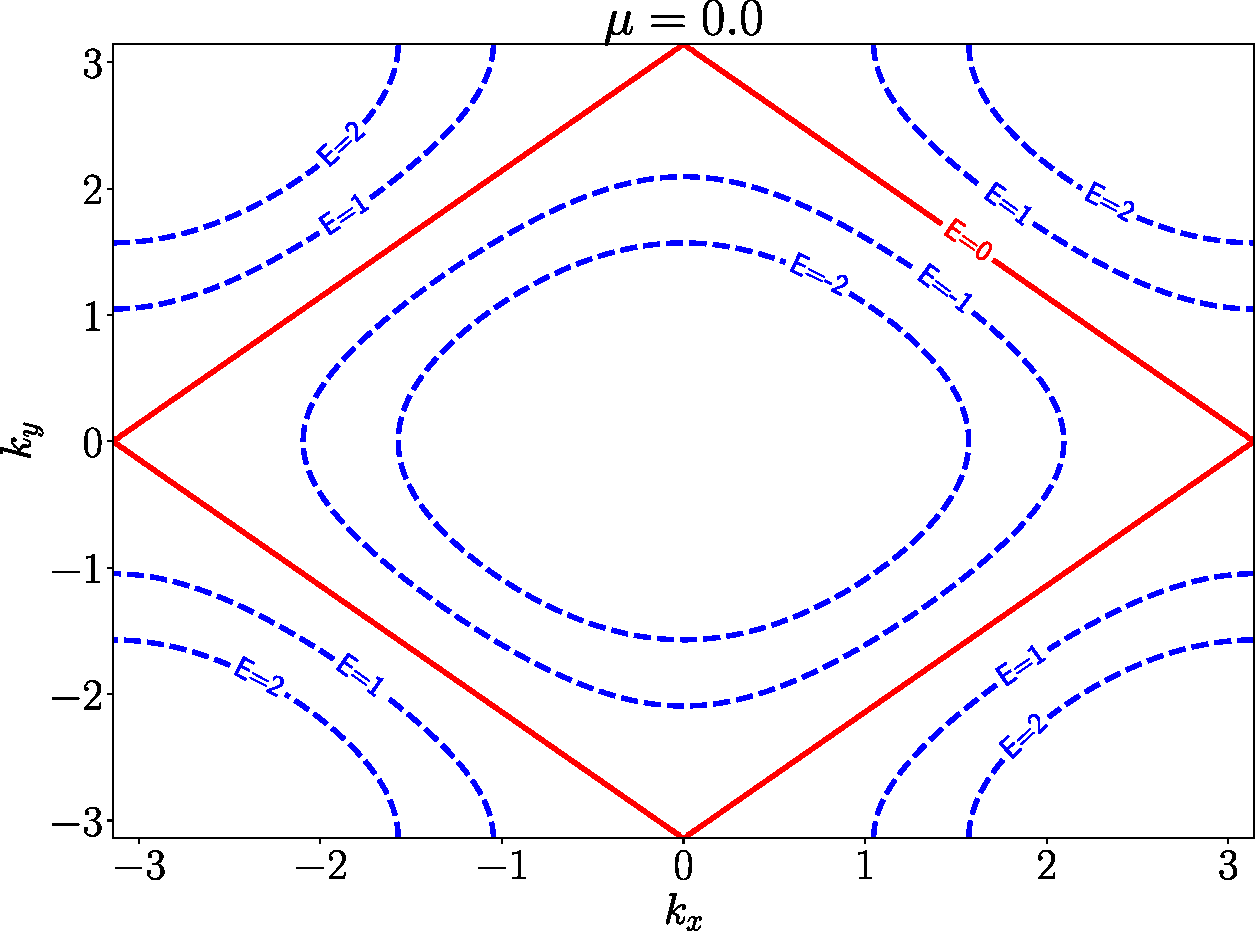
\includegraphics[width=0.8\textwidth]{./contours.pdf}
	\caption{Contours of constant energy on the 2D tight-binding lattice model, at half-filling \((\mu = 0)\). The red lines form the Fermi surface, while the blue lines form other contours.}
\end{figure}

\newpage
\subsection*{Half-filling}
\begin{minipage}{0.5\textwidth}
	The case of \(\mu=0\) is often referred to as half-filling, because at this parameter value, the Hamiltonian is particle-hole symmetric. This means that the Hamiltonian remains invariant under a particle-hole transformation. To see this on the 2D lattice, we visualize the lattice as the sum of two sub-lattices, A and B. A site on sublattice A (pink in figure) only has sites of sublattice B (green in figure) as its nearest-neighbour, and vice-versa. We will represent the Fermionic operators for sublattice \(A\) with \(a,a^\dagger\) ad those of sublattice \(B\) with \(b, b^\dagger\).
\end{minipage}
\hspace*{\fill}
\begin{minipage}{0.4\textwidth}
	\centering
	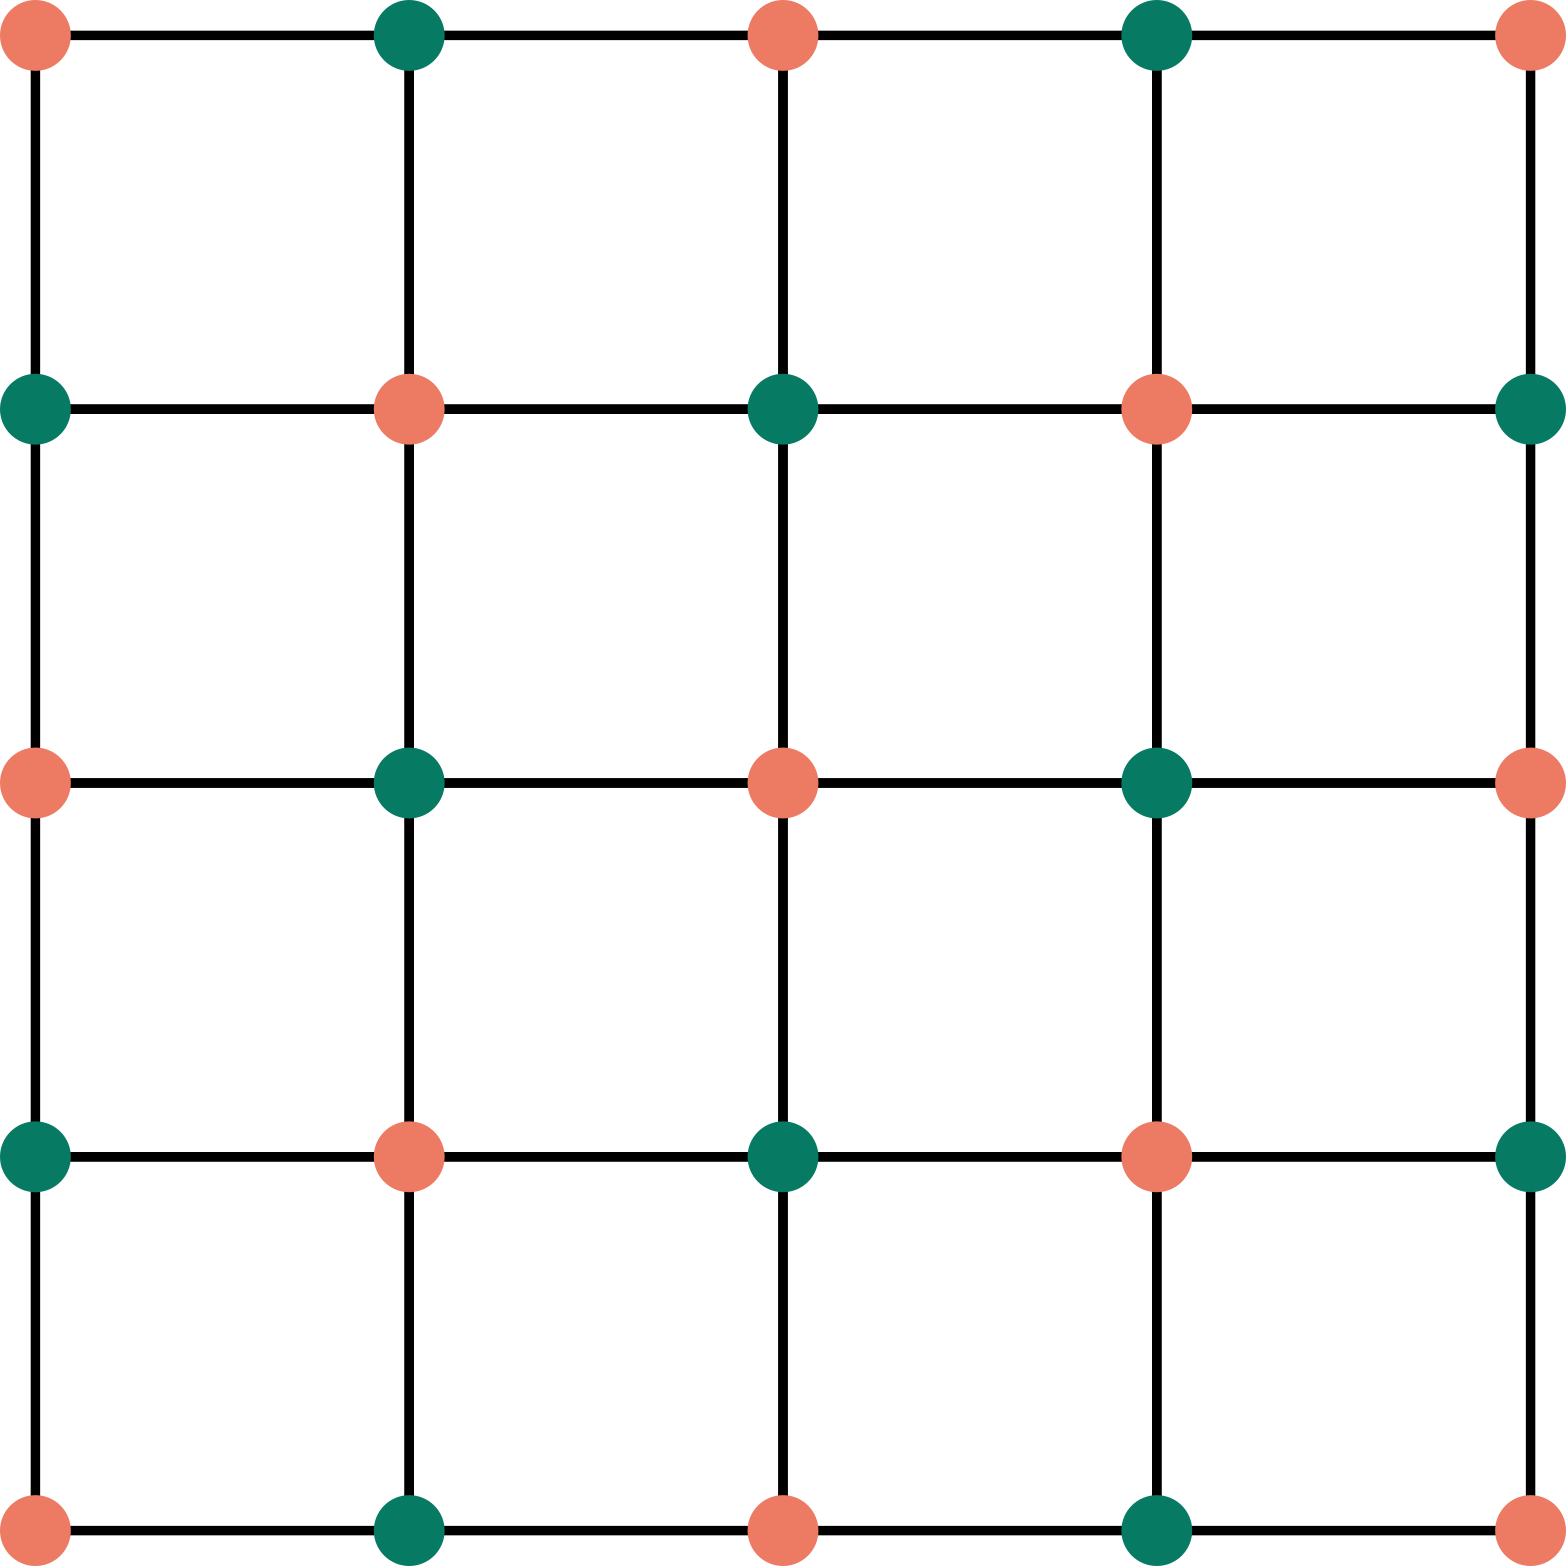
\includegraphics[width=0.8\textwidth]{./sublattice.png}
	\captionof{figure}{2D lattice composed of two sublattices. Pink indicates sites on sublattice A and green indicates sites on sublattice B.}
\end{minipage}
\\\\
With this in mind, the tight-binding Hamiltonian can be written as
\begin{equation}\begin{aligned}
	H = -t\sum_{i \in A}\sum_{j \in \text{NN of i}} \sum_\sigma\left(a^\dagger_{i \sigma}b_{j\sigma} + \text{h.c.}\right) - \mu \hat N
\end{aligned}\end{equation}
Now we define a particle-hole transformation \(a \to a^\dagger, b \to -b^\dagger\). The hopping part remains unchanged by this transformation:
\begin{equation}\begin{aligned}
	a^\dagger_{i \sigma}b_{j\sigma} + b^\dagger_{j\sigma}a_{i\sigma} \to -a_{i\sigma}b^\dagger_{j\sigma} - b_{j\sigma}a^\dagger_{i\sigma} = a^\dagger_{i \sigma}b_{j\sigma} + b^\dagger_{j\sigma}a_{i\sigma}
\end{aligned}\end{equation}
The total number part transforms as
\begin{equation}\begin{aligned}
	\mu \hat N = \mu\left(\sum_{i\in A,\sigma}a^\dagger_{i\sigma}a_{i\sigma} + \sum_{j\in B,\sigma}b^\dagger_{j\sigma}b_{j\sigma}\right) \to -\mu\hat N + \text{constant}
\end{aligned}\end{equation}
This term will be invariant when
\begin{equation}\begin{aligned}
	\mu \hat N = -\mu\hat N \implies \mu = 0
\end{aligned}\end{equation}

\newpage
\subsection*{Problem 1. Electronic differentiation and nesting at half-filling}
\begin{minipage}{0.5\textwidth}
	The half-filled Fermi surface has two sets of high-symmetry points. The points at the four corners are referred to as the \textit{antinodal points}, while those at the centers of the four arms are referred to as the \textit{nodal points}. The dispersion behaves differently near the two sets of points: near the nodes, it is massless Dirac-like, while near the antinodes, it becomes hyperbolic.
\end{minipage}
\hspace*{\fill}
\begin{minipage}{0.4\textwidth}
	\centering
	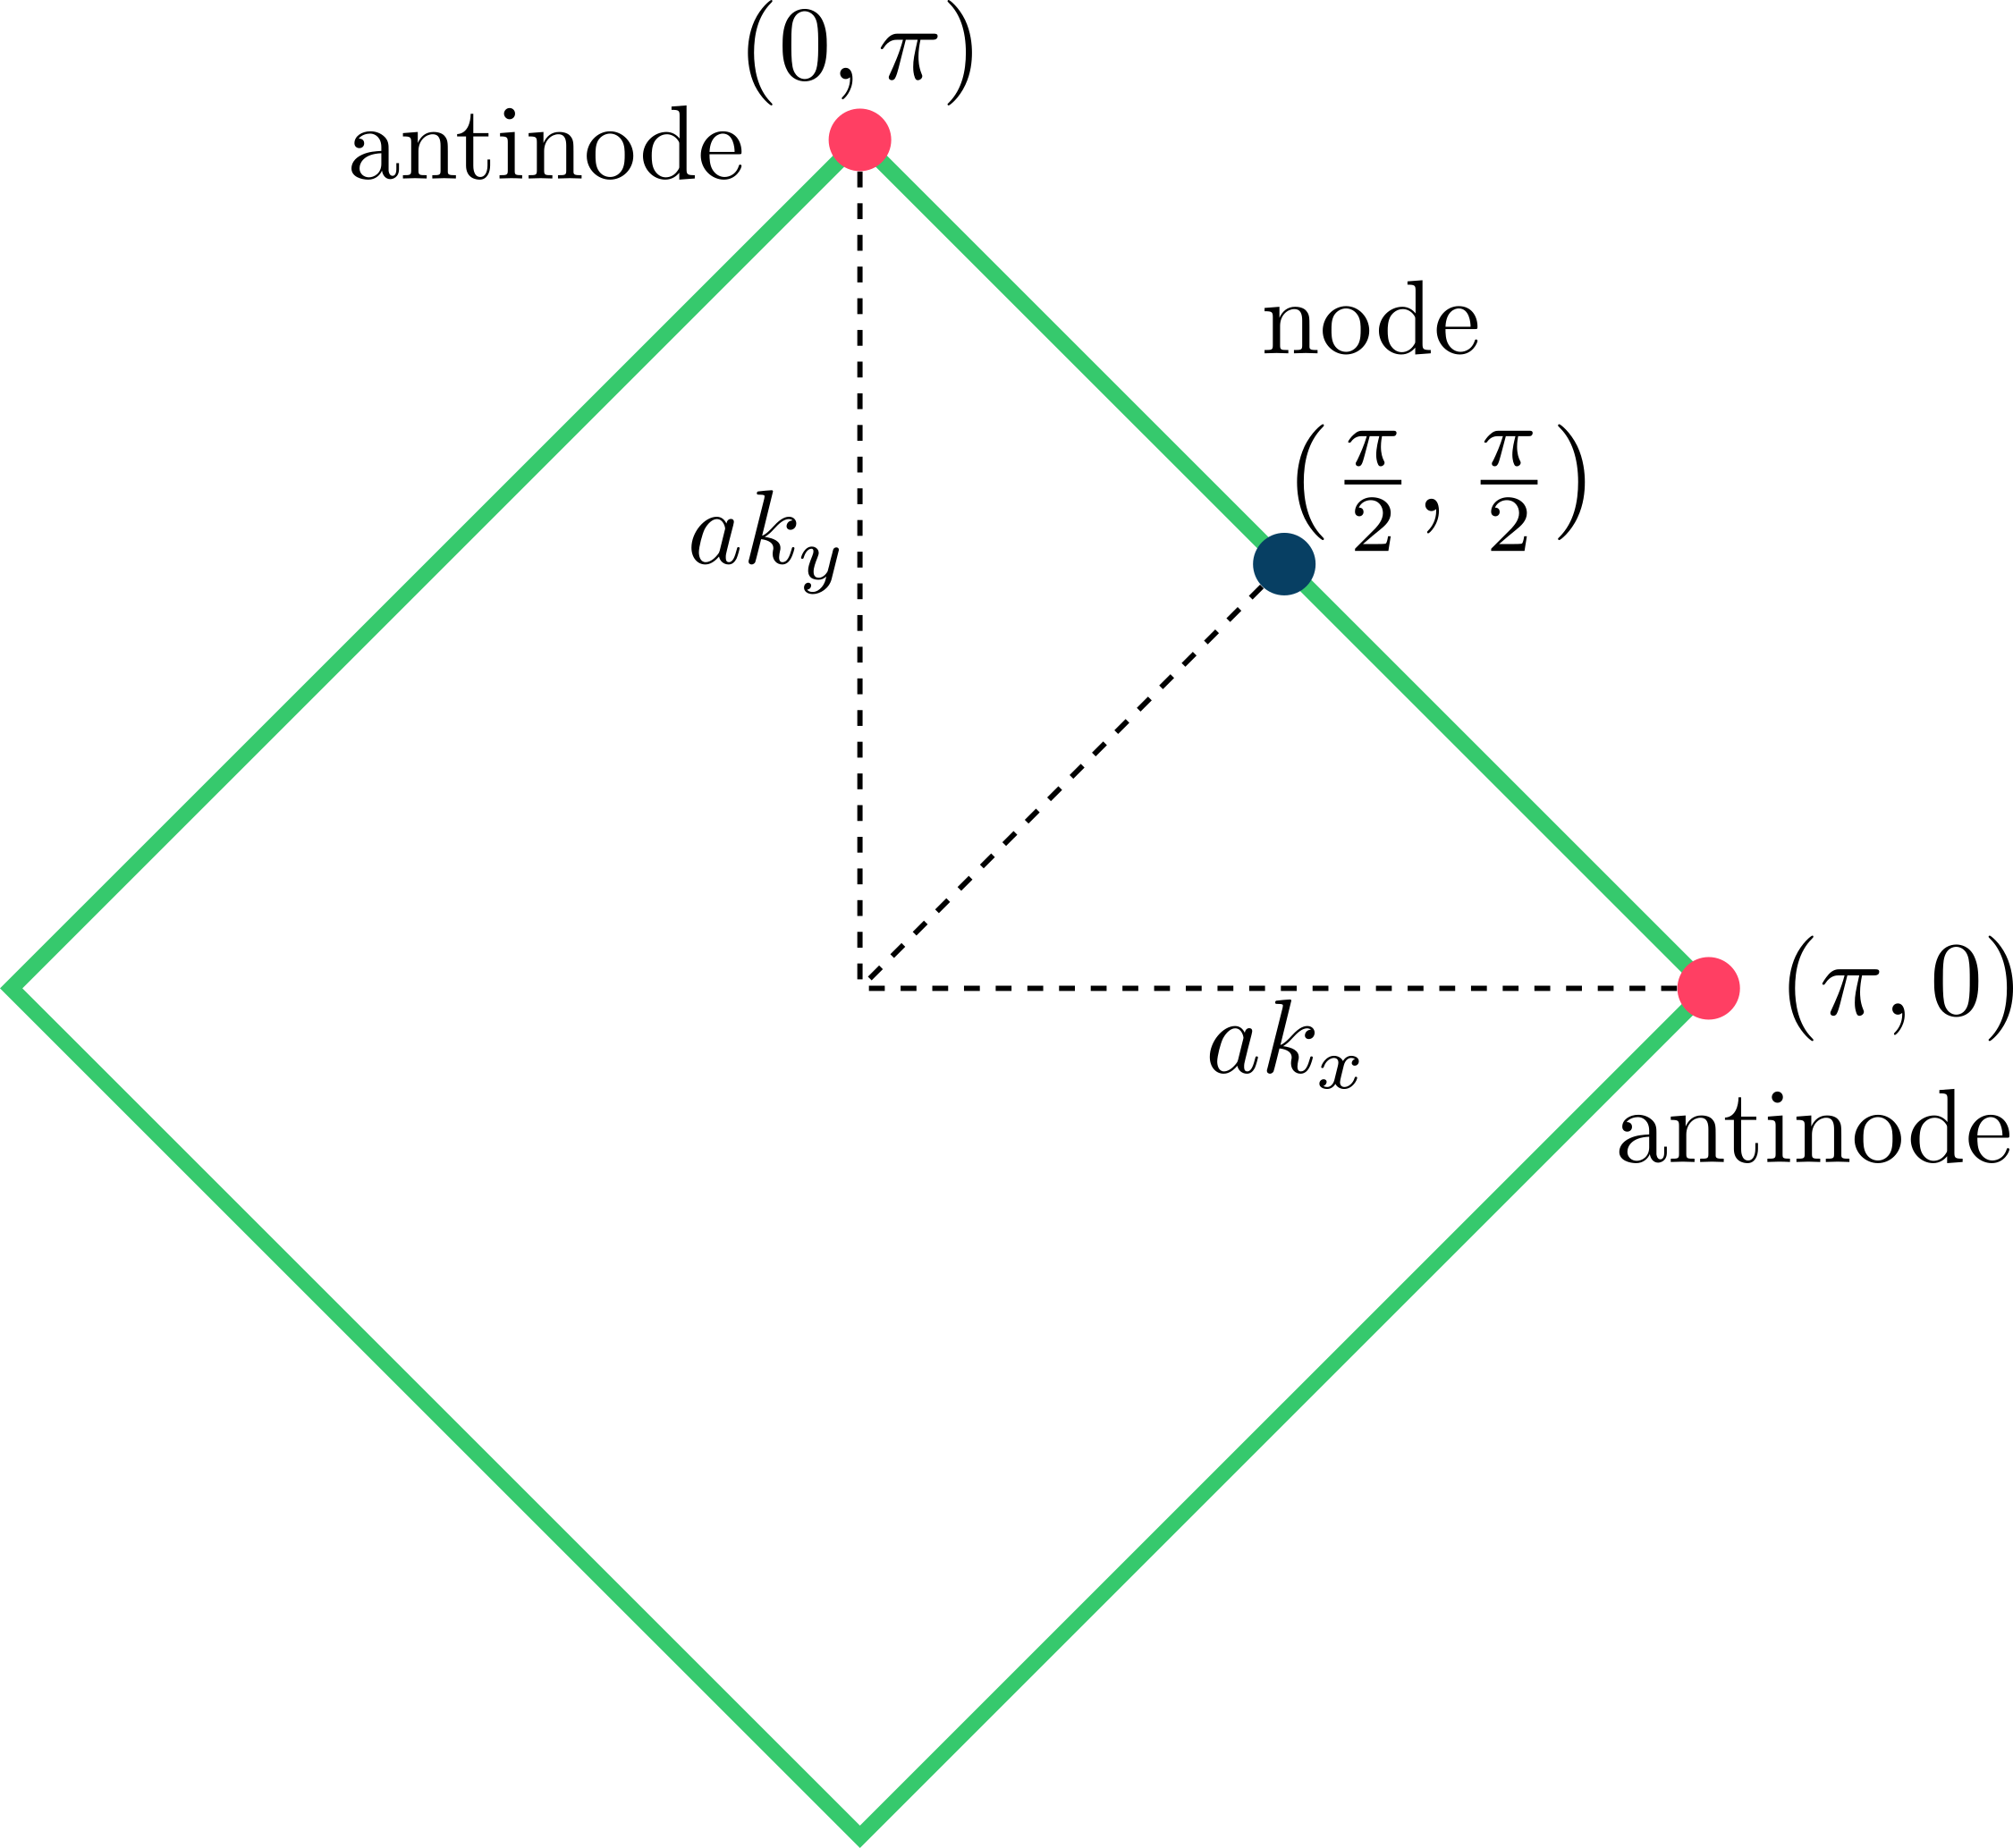
\includegraphics[width=\textwidth]{./Fsurf.png}
\end{minipage}
\\\\
\begin{equation*}\begin{aligned}
	\text{antinodes } \to \left(ak_x, ak_y\right) = \begin{cases}
\left(0, \pi \right), \left(\pi, 0 \right)\\
\left(0, -\pi \right), \left(-\pi, 0\right)
	\end{cases}\\
		\text{nodes } \to \left(ak_x, ak_y\right) = \begin{cases}
		\left(\frac{\pi}{2}, \frac{\pi}{2} \right), \left(-\frac{\pi}{2}, -\frac{\pi}{2}\right)\\
		\left(\frac{\pi}{2}, -\frac{\pi}{2} \right), \left(-\frac{\pi}{2}, \frac{\pi}{2}\right)
	\end{cases}
\end{aligned}\end{equation*}
\paragraph{Questions:}
\begin{itemize}
	\item Write down the dispersion at half-filling by substituting \(\mu=0\) and also assume \(t=1\) for simplicity. 
	\item Expand this dispersion in a Taylor series  about \(k_x = k_y = \frac{\pi}{2}\) to get the behaviour around the nodal point. You should obtain a linear form.
	\item Also expand this dispersion in a Taylor series  about \(k_x = \pi, k_y = 0\) to get the behaviour around the antinodal point. You should obtain a hyperbolic form.
	\item Nesting refers to the phenomenon where a single vector in momentum space connects large parts of the Fermi surface. Can you find the momentum vector that connects either of the two parallel arms of the Fermi surface?
\end{itemize}
\newpage
The dispersion \(\epsilon_k = -2t\left(\cos(k_x a_x) + \cos(k_y a_y)\right)\) near the nodes and antinodes can be obtained by expanding the cosines in Taylor series about those points. Near the nodes, we have
\begin{equation}\begin{aligned}
	ak \sim \frac{\pi}{2} \implies \cos(ak) \sim \left(ak - \frac{\pi}{2}\right)(-1)
\end{aligned}\end{equation}
which gives
\begin{equation}\begin{aligned}
	\epsilon_k \vert_\text{node} \sim 2t \left(a_x k_x + a_y k_y\right)
\end{aligned}\end{equation}
\textit{The dispersion becomes linear near the nodes.} Near one of the antinodes, we have \(k_x a_x \sim \pi, k_y a_y \sim 0\), so
\begin{equation}\begin{aligned}
	\cos (a_x k_x) &\sim -1 + \frac{1}{2}\left( \pi - a_x k_x \right)^2\\
	\cos (a_y k_y) &\sim 1 - \frac{1}{2}\left(a_y k_y \right)^2\\
\end{aligned}\end{equation}
such that
\begin{equation}\begin{aligned}
	\epsilon_k \vert_\text{antinode} \sim t \left[\left(a_y k_y \right)^2 - \left( \pi - a_x k_x \right)^2\right]
\end{aligned}\end{equation}
which shows that the \textit{dispersion becomes hyperbolic near the antinodal points}.
\\\\
\textit{Nesting} refers to the situation where a single vector in the reciprocal lattice vector space (momentum space) connects large patches of the Fermi surface. For the case of a half-filled Fermi surface, the momentum vector \(\vec Q = \frac{1}{a}\left( \pi, \pi\right)\) connects two whole arms of the Fermi surface. If there is some scattering mechanism in the theory that connects states lying at momenta \(k\) and \(k+Q\), there will be terms in perturbation theory that go as
\begin{equation}\begin{aligned}
	\frac{1}{\xi_{\vec k} - \xi_{\vec k + \vec Q}}
\end{aligned}\end{equation}
Since \(\vec Q\) connects a large number of points on the Fermi surface, there will be many choices such that \(\vec k\) and \(\vec k + \vec Q\) lie on the Fermi surface, and are hence degenerate states. The presence of the nesting vector \(\vec Q\) thus leads to a very high static structure factor for such scattering processes between degenerate states.

\newpage
\subsection*{Problem 2. van Hove singularity: Logarithmic divergence of the density of states}
The DOS at an energy $E$ is given by
\begin{equation}\begin{aligned}
	\rho(E) = \frac{1}{4\pi^2}\int_{S(E)} \frac{dS}{|\vec \nabla \epsilon_{\vec{k}}|}
\end{aligned}\end{equation}
The integral is over the surface \(S(E)\) of constant energy $E$. Henceforth, for simplicity, we will assume \(\mu=0\) and \(a=1\). 
\paragraph{Questions:}
\begin{itemize}
	\item Write down the dispersion upto second order near the antinodal point \(k_x, k_y = \pi, 0\). Then calculate the velocity \(|\vec \nabla \epsilon_{\vec{k}}|\).
	\item Since the integration is carried out over a constant energy surface, we can equate the dispersion to the energy \(E\) which we assume to be positive. In this fashion, obtain an equation between \(k_x\) and \(k_y\). Think of a parametrization \(\pi - k_x = f(\phi), k_y = g(\phi)\) that reduces the two variables \(k_x\) and \(k_y\) to a single variable \(\phi\). [\textit{Hint: Think of hyperbolic functions}]
	\item Express the velocity calculated previously purely in terms of \(\phi\). Also calculate the arc length \(dS = \sqrt{dk_x^2 + dk_y^2}\) in terms of \(\phi\). Substitute these into \(\rho(E)\) to obtain an integral purely in terms of \(\phi\). Convince yourself that the actual integral is double of what you currently have, because \(k_y\) is forced to have a specific sign in this parametrization. The opposite sign gives exactly the same contribution.
	\item With the factor of \(2\), evaluate the integral between the limits \(\phi_1\) and \(\phi_0\). These limits can be obtained by substituting the boundary values of \(k_y\) into the equation \(g(\phi) = k_y\). Now take the limit of \(E \to 0^+\) to simplify the expression. [\textit{Hint: }\(\lim_{x \to \infty} \sinh(x) = \ln 2x\)]
\end{itemize}
\newpage


Near the antinodal point \(\left(\pi, 0\right) \), we can approximate the dispersion as
\begin{equation}\begin{aligned}
	\epsilon_{\vec k} = t\left[k_y^2 - \left( \pi - k_x \right) ^2\right] 
\end{aligned}\end{equation}
Since we are integrating over a constant energy surface \(E \), we can write
\begin{equation}\begin{aligned}
	k_y^2 - \left( \pi - k_x \right)^2 = \frac{E}{t} = R^2
\end{aligned}\end{equation}
We assumed here that \(E > 0\). The hyperbolic nature of the equation suggests a parametrization of the form
\begin{equation}\begin{aligned}
	k_y = R\sinh \phi, &&\pi - k_x = R\cosh \phi
\end{aligned}\end{equation}
This allows us to parametrize the integral using just one variable \(\phi\). The gradient of the dispersion is
\begin{equation}\begin{aligned}
	|\vec \nabla \epsilon_{\vec{k}}| = \sqrt{\left(\frac{\partial{\epsilon_{\vec k}}}{\partial{k_x}}\right)^2 + \left(\frac{\partial{\epsilon_{\vec k}}}{\partial{k_y}}\right)^2} = 2t\sqrt{\left(\pi - k_x\right)^2 + k_y^2} = 2tR\sqrt{\cosh^2\phi + \sinh^2\phi}
\end{aligned}\end{equation}
and the arc length can be written as
\begin{equation}\begin{aligned}
	dS = \sqrt{(dk_x)^2 + (dk_y)^2} = Rd\phi\sqrt{\cosh^2\phi + \sinh^2\phi}
\end{aligned}\end{equation}
The integral can now be written purely in terms of \(\phi\):
\begin{equation}\begin{aligned}
	\rho(E) = \frac{1}{4\pi^2}\frac{1}{2t}\int d\phi = \frac{1}{4\pi^2}\frac{1}{2t}\left[\phi_1 - \phi_0\right] 
\end{aligned}\end{equation}
Note that we have accounted for only half of the integration space currently. To see this, consider the case when we are integrating over the half-filled Fermi surface, so we can assume \(\sinh \phi = \pi - \cosh \phi\). This however, would just produce the top half of the diamond, because \(\sinh \phi\) is always positive here. To get the other half, we need the other parametrization choice of 
\begin{equation}\begin{aligned}
	k_y = -R\sinh \phi, &&\pi - k_x = R\cosh \phi
\end{aligned}\end{equation}
Since both \(dS\) and the gradient involve only even functions, they will not be affected and the total integral will just be twice of what we currently have.
\begin{equation}\begin{aligned}
	\rho(E) = \frac{1}{4\pi^2}\frac{1}{t}\left[\phi_1 - \phi_0\right] 
\end{aligned}\end{equation}
We now need to figure out the integration limits \(\phi_1\) and \(\phi_0\). Since we are integrating over the first Brillouin zone, \(k_y\) ranges from \(-\pi \to \pi\), such that \(\phi\) ranges from
\begin{equation}\begin{aligned}
	\phi_0 = \sinh^{-1}\frac{-\pi}{R} = -\sinh^{-1}\frac{\pi}{R}\to \phi_1 =\sinh^{-1}\frac{\pi}{R}
\end{aligned}\end{equation}
This gives
\begin{equation}\begin{aligned}
	\rho(E) = \frac{1}{2t\pi^2}\sinh^{-1}\sqrt\frac{2t\pi^2}{E}
\end{aligned}\end{equation}
We are interested in \(E \to 0^+\), so the term in the square root will be very large. This allows us to approximate the sinh inverse as a logarithm:
\begin{equation}\begin{aligned}
	\sinh^{-1}(x) = \ln\left( x + \sqrt{x^2 + 1} \right) \implies \lim_{x \to \infty} \sinh^{-1}(x) = \ln 2x
\end{aligned}\end{equation}
For the DOS, this means
\begin{equation}\begin{aligned}
	\rho(E \to 0^+) \sim \frac{1}{2t\pi^2} \ln \sqrt\frac{4t\pi^2}{E} = \frac{1}{4t\pi^2}\left(\ln 4t\pi^2 - \ln E\right) 
\end{aligned}\end{equation}
The logarithmic divergence in the density of states is visible now. The presence of a large number of states, specially close to the Fermi surface, results in increased correlation between the electrons and might lead to instablities because of the increased scattering near the singularity.

\newpage
\subsection*{References}
\begin{itemize}
	\item Solid State Physics, \textit{Ashcroft Mermin}
	\item The Oxford Solid State Basics, \textit{Steven H. Simon}
	\item An Introduction to the Hubbard Hamiltonian, \textit{Richard T. Scalettar}
\end{itemize}
\end{document}
